\documentclass{beamer}
\usetheme{Boadilla}
\usecolortheme{whale}
\usepackage{comment}
\usepackage{ragged2e}
\usepackage{amsmath}
\usepackage{dcolumn}
\usepackage{booktabs}
\usepackage{pdflscape}
\usepackage{graphicx}
\usepackage{placeins}
\usepackage{dcolumn}
\usepackage{xcolor}
\usepackage{booktabs}
\linespread{1.5}
\usepackage{subcaption}
\usepackage{amsmath}
\usepackage{hyperref}
\usepackage{multirow}
\usepackage{tikz}
\usepackage[title]{appendix}
\usetikzlibrary{decorations.pathreplacing}
\usepackage{booktabs}
\usepackage{tabularx}
%\usepackage{xepersian}
%\settextfont{XB Zar}
%\setdigitfont{XB Zar}


\renewcommand{\today}{\ifcase \month \or January\or February\or March\or %
April\or May \or June\or July\or August\or September\or October\or November\or %
December\fi, \number \year} 


\AtBeginSection[]
{
    \begin{frame}
        \frametitle{Table of Contents}
        \tableofcontents[currentsection]
    \end{frame}
}

\title[Price Synchronicity]{\large Large controlling shareholders and stock price synchronicity\footnote{ \tiny Jornal of Banking \& Finance - 2014}}
\subtitle{\scriptsize Sabri Boubaker \qquad Hatem Mansali \qquad Hatem Rjiba }
\author[Aghajanzadeh]{S.M. Aghajanzadeh A. }
\institute[]{Tehran Institute for Advanced Studies }
\centering

\begin{document}

{\maketitle}
\small

\section{Introduction}
\begin{frame}
	\begin{itemize}
		\scriptsize
		\item Stock prices move together depends on the relative amounts
		of firm-specific and market-level information impounded into
		stock prices.  [Roll (1988)]
		\item Morck et al. (2000) show that R-squared
		is lower in countries that properly protect investors’ property
		rights
	\end{itemize}
\begin{columns}
	\column{0.48\textwidth}
	\begin{block}{\footnotesize Stock price synchronicity}
			\begin{itemize}
			\tiny
			\item Efficient capital allocation (Pindyck and Rotemberg, 1993; Wurgler, 2000)
			\item  Analyst
			activity (Piotroski and Roulstone, 2004; Chan and Hameed, 2006)
			\item Earnings informativeness (Durnev et al., 2003)
			\item Corporate transparency (Jin and Myers, 2006)
			\item Voluntary disclosure (Haggard et al.,
			2008)
			\item  Earnings management (Hutton et al., 2009)
			\item audit quality
			(Gul et al., 2010)
			\item The adoption of International Financial Reporting Standards (Kim and Shi, 2012)
		\end{itemize}
	\end{block}

	\column{0.48\textwidth}
	\setbeamercolor{block title}{fg=white,bg=red!85!black}
	\setbeamercolor{block body}{bg=block title.bg!10!bg}
	
	
		\begin{block}{\footnotesize Ownership structure }
		\begin{itemize}
			\tiny
			\item  the distribution of cash flow and voting
rights shapes the outcome of financial reporting procedures.(Ball et al., 2003) 

\item  Earnings management (Warfield et al., 1995)
\item  Earnings informativeness (Fan and Wong, 2002)
\item  Analyst following (Lang et al.,
2004; Boubaker and Labégorre, 2008)
\item  Accounting conservatism
(Lafond and Roychowdhury, 2008)
\item  The cost of corporate
borrowing (Boubakri and Ghouma, 2010; Lin et al., 2011)
		\end{itemize}
	\end{block}
\end{columns}




\end{frame}

\begin{frame}{This Paper}
	\begin{itemize}
		\item Brings together these two strands of literature
		\begin{block}{Question}
			Does ownership structure matters in explaining the synchronicity of stock price movements?
		\end{block}
	\item  Two
	important corporate governance characteristics
	\begin{itemize}
		\item  Ultimate cash flow rights of controlling shareholders
		\item The separation of voting and
		cash flow rights
	\end{itemize}
	\end{itemize}
\end{frame}


\section{Hypothesis development}
\begin{frame}{Excess control and stock price synchronicity}
\begin{itemize}
	\scriptsize
	\item Grossman and Hart (1988) demonstrate that deviation from the
	one share–one vote rule maximizes the benefits of control for the
	controlling party relative to security holders and thus may not be
	socially optimal. 
	\item Shleifer and Vishny (1997) argue that as ownership increases beyond a certain level, insiders gain almost full control of the firm and may prefer to extract private benefits of control
	that do not accrue to minority shareholders. This problem is more
	pronounced when control rights exceed cash flow claims
	(Claessens et al., 2002). 
	\item Bebchuk (1999) demonstrates that when
	the private benefits of control are sizable, controlling shareholders strive to maintain a lock on the firm to maximize rent extraction.
\end{itemize}
\begin{block}{Hypothesis 1}
	Stock price synchronicity increases with the excess control of
	the ultimate controlling shareholder
\end{block}
\end{frame}

\begin{frame}{Ownership concentration and stock price synchronicity}
	\begin{itemize}
		\scriptsize
		\item The literature suggests that ownership concentration helps mitigate the conflict of interests between controlling and minority
		shareholders
		\item Large shareholders are less inclined to conceal information when they hold
		large ownership stakes in a firm. Rather, they have incentives to
		disseminate more and better firm-specific information
	\end{itemize}
\begin{block}{Hypothesis 2}
	Stock price synchronicity decreases with the cash flow rights
	of the ultimate controlling shareholder
\end{block}
\end{frame}
\section{Data and variable construction}
\begin{frame}{Data and variable construction}
\begin{itemize}
	\item Data
		\begin{itemize}
			\scriptsize
		\item French listed firms during 1998 –
		2007 
		\item Non-financial firms
		
	\end{itemize}
\item Ownership structure variables
\begin{itemize}
	\scriptsize
	\item Ultimate Owner: A shareholder who maintains at least 10\% of a firm’s voting rights without being controlled by anyone else.
	\item 
	Ultimate cash flow rights of the
	largest controlling shareholder (UCF) as the sum of the products of
	direct cash flow rights along the different ownership chains and its
	ultimate control rights as the sum of the weakest links across all these
	chains.
	\item  Excess control (Excess) is defined as the difference between the	ultimate control and cash flow rights of the largest controlling shareholder, scaled by ultimate control rights (UCO  UCF)/UCO).
\end{itemize}
\end{itemize}
\end{frame}
\begin{frame}{Stock price synchronicity}
\begin{itemize}
	\item  Estimating the following modified
	market model for each firm–year
	\begin{equation*}
		RET_{i,w} = \alpha + \beta_1 MKRET_{w-1}  + \beta_2 MKRET_{w}  + \beta_3 INDRET_{i,w-1}  + \beta_4 INDRET_{i,w}
	\end{equation*}
	\item  R-squared value obtained from the above regression
	\begin{equation*}
		SYNCH = log(\frac{R^2_{i,t}}{1-R^2_{i,t}})
	\end{equation*}
\end{itemize}
\end{frame}
\begin{frame}{Summary statistics}
	\begin{figure}
		\centering
		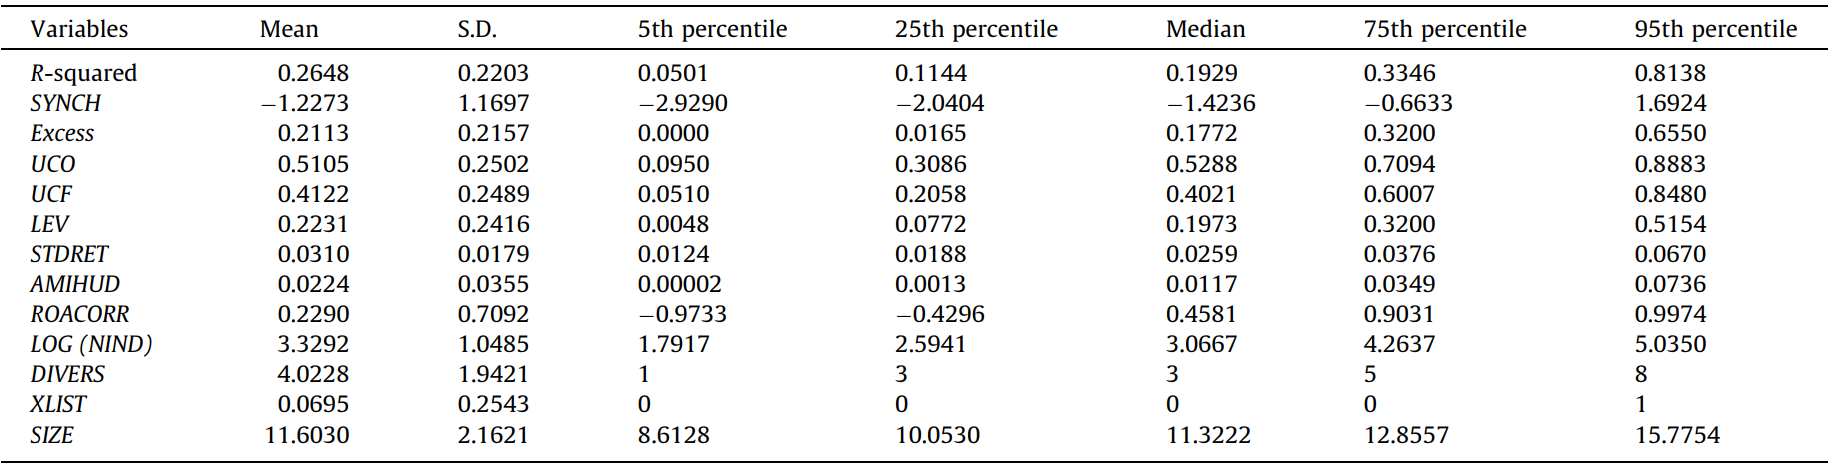
\includegraphics[width=\linewidth]{t2}
		\label{fig:t2}
	\end{figure}
	
\end{frame}
\section{Regression results}
\begin{frame}{Model}
	\begin{itemize}
		\item  Regression model
		 \begin{equation*}
			\begin{split}
				\text{SYNCH}_{i,t} & =  \beta_0 + \beta_1\text{Excess}_{i,t}
			+ \beta_2\text{UCF}_{i,t}\\
			& 
			+ \sum_{k}\beta_k \text{Control}_{i,t}^k +
			\text{IndustryDummies} + \text{YearDummies} + \varepsilon_{i,t}
			\end{split}
		\end{equation*}
		\begin{itemize}
		\tiny
		\item $ \text{Excess} = (\text{cr} - \text{cfr})/\text{cr} $
		\item $ \text{ExcessDiff} = \text{cr} - \text{cfr} $
		\item $ \text{ExcessDummy} = \left\{\begin{array}{ll}
			1 & \text{cr} - \text{cfr}>0\\
			0 & \text{cr} - \text{cfr}\leq 0
		\end{array}\right.  $
		\item $ \text{ExcessHigh} = \left\{\begin{array}{ll}
			1 & \text{Excess}>\text{Median}(\text{Excess})\\
			0 & \text{Excess}\leq \text{Median}(\text{Excess})
		\end{array}\right.  $
	\end{itemize}
\item Pooled OLS
regression with industry and year fixed effects. 
\item Standard errors are corrected for firm-level clustering

	\end{itemize}
\end{frame}

\begin{frame}
		\begin{figure}
		\centering
		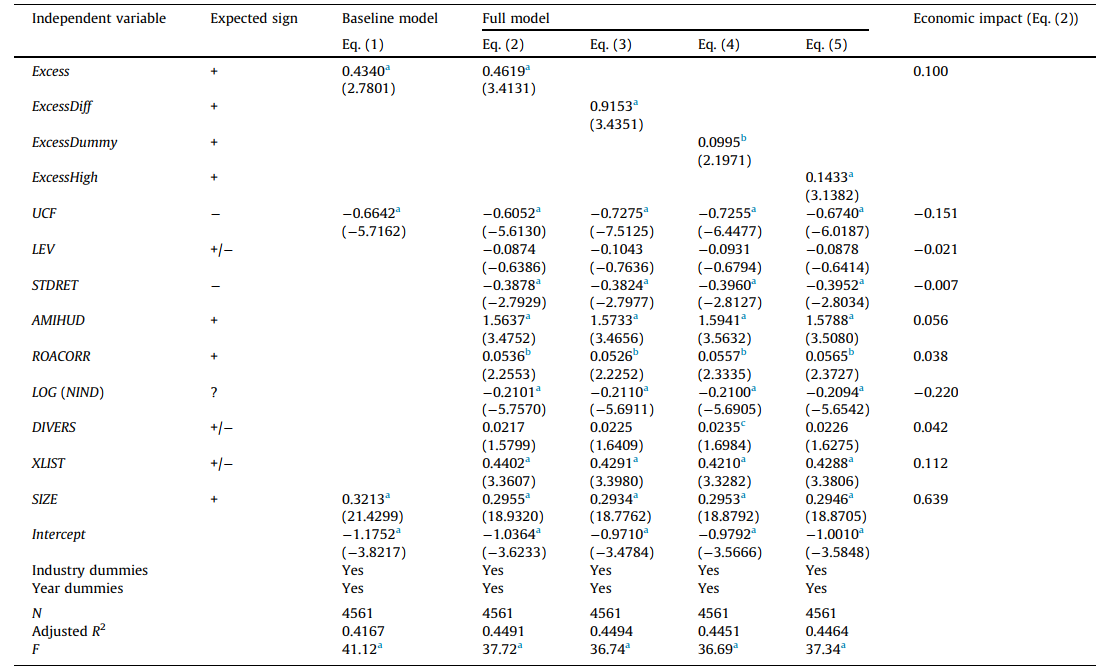
\includegraphics[width=\linewidth]{t4}
		\label{fig:t4}
	\end{figure}
\end{frame}
\begin{frame}{Cash Risk}
	\begin{itemize}
		\item Jin and Myers (2006) demonstrate that stockpiling bad news is not everlasting but, instead, continues only up to a certain threshold, above which all bad news is suddenly released, resulting in a significant downward stock price revision, that is, a stock price crash.
		\item  Regression model
		\begin{equation*}
			\begin{split}
				\text{CrashRiski}_{i,t} & =  \beta_0 + \beta_1\text{Excess}_{i,t}
				+ \beta_2\text{UCF}_{i,t}\\
				& 
				+ \sum_{k}\beta_k \text{Control}_{i,t}^k +
				\text{IndustryDummies} + \text{YearDummies} + \varepsilon_{i,t}
			\end{split}
		\end{equation*}
	\item Cash Risk: an dummy variable that equals to one if the firm exhibits within its fiscal year a weekly
	residual return below k-standard deviations of the mean weekly residual returns; zero otherwise
	\end{itemize}
\end{frame}

\begin{frame}
	\begin{figure}
		\centering
		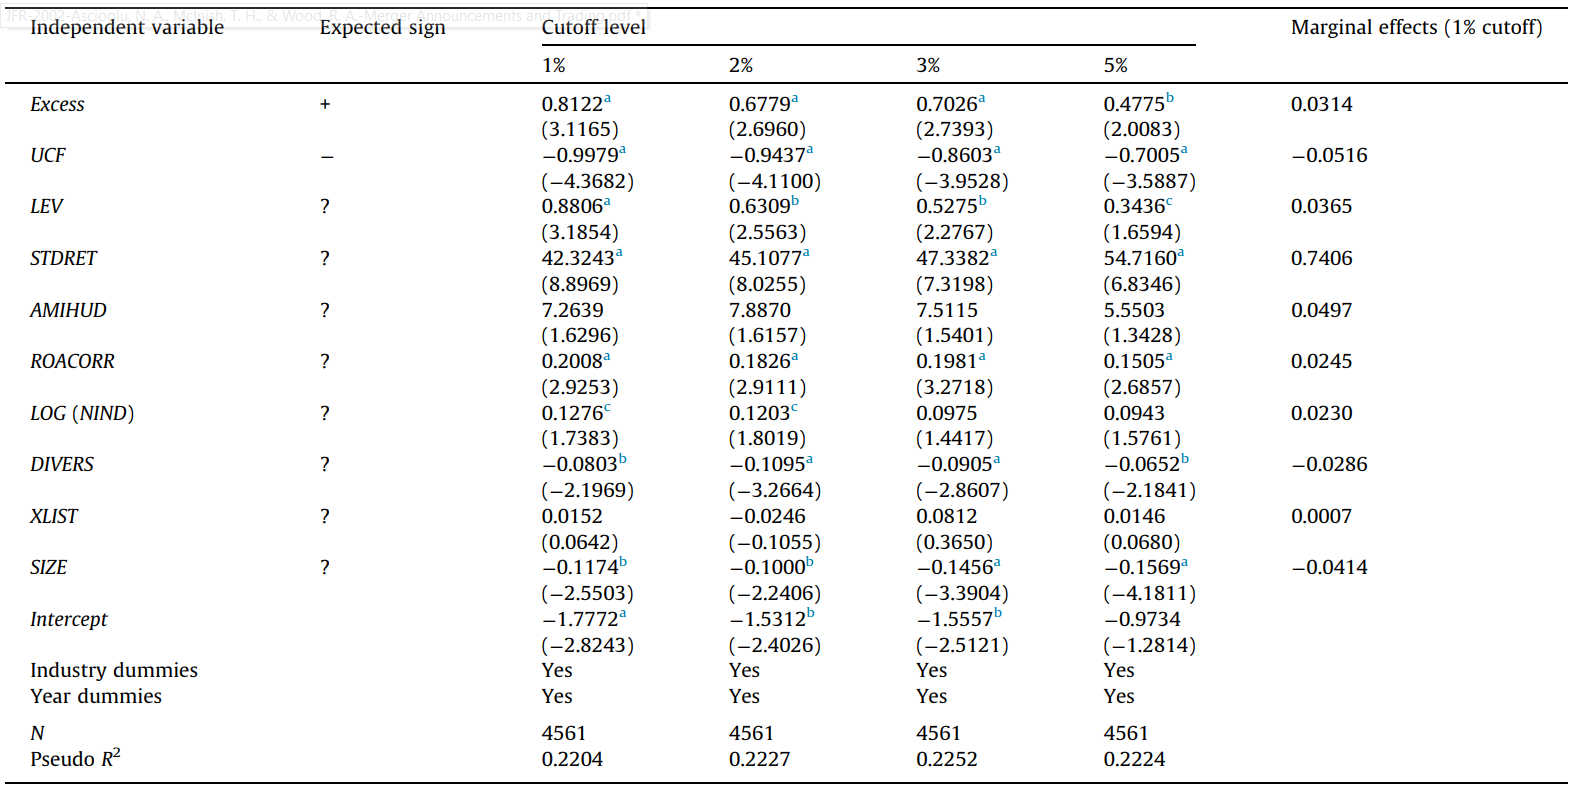
\includegraphics[width=\linewidth]{t6}
		\label{fig:t6}
	\end{figure}
\end{frame}

\begin{frame}{The impact of the FSL of August 1, 2003}
		\begin{figure}
		\centering
		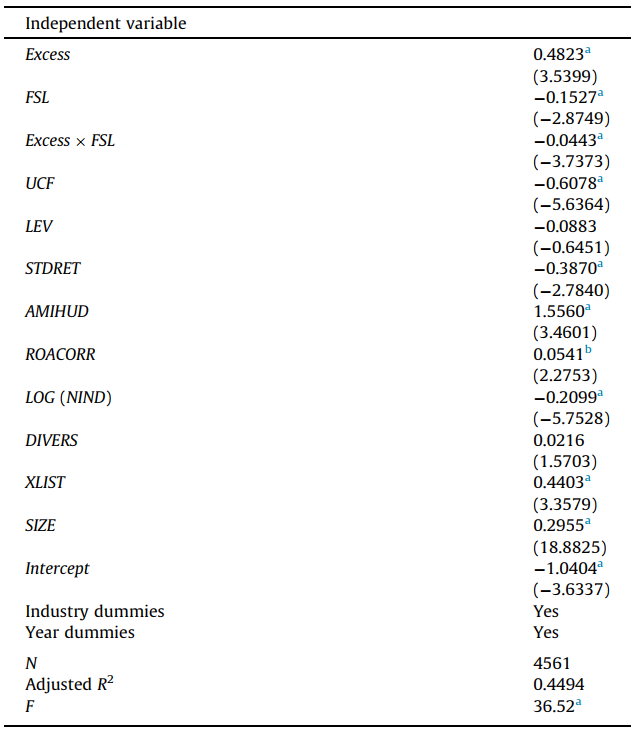
\includegraphics[width=0.7\textheight]{t8}
		\label{fig:t8}
	\end{figure}
\end{frame}

\begin{frame}{Product market competition}
	\begin{figure}
		\centering
		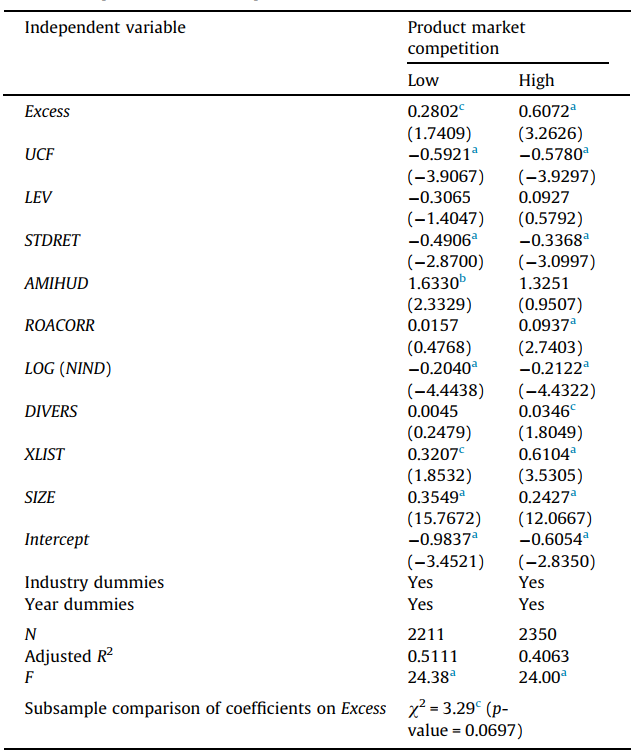
\includegraphics[width=0.7\textheight]{t9}
		\label{fig:t9}
	\end{figure}
\end{frame}





\section{Conclusion}
\begin{frame}{Conclusion}
	\begin{itemize}
		\item The separation of
		control and cash flow rights is positively associated with the
		amount of industry- and market-level information incorporated
		into stock prices
		\item 
		Firm with 
		substantial control–ownership wedge is more prone to crashes,
		which is consistent with the notion that controlling shareholders
		are able to hide information only up to a certain threshold, upon
		which all bad news is suddenly disclosed
		\item Stock prices are less synchronous and less likely to crash when controlling shareholders
		own a large fraction of cash flow rights
	\end{itemize}
\end{frame}
\section{Iran's Data}
\begin{frame}
	\begin{table}[htbp]
		\centering
		\resizebox{0.7\textheight}{!}{
			{
\def\sym#1{\ifmmode^{#1}\else\(^{#1}\)\fi}
\begin{tabular}{l*{8}{c}}
\hline\hline
                    &\multicolumn{8}{c}{Synchronicity}                                                                                                                                              \\\cmidrule(lr){2-9}
                    &\multicolumn{1}{c}{(1)}         &\multicolumn{1}{c}{(2)}         &\multicolumn{1}{c}{(3)}         &\multicolumn{1}{c}{(4)}         &\multicolumn{1}{c}{(5)}         &\multicolumn{1}{c}{(6)}         &\multicolumn{1}{c}{(7)}         &\multicolumn{1}{c}{(8)}         \\
\hline
Excess              &                     &      -0.899\sym{**} &      -0.557\sym{*}  &                     &                     &                     &                     &                     \\
                    &                     &     [-3.22]         &     [-2.10]         &                     &                     &                     &                     &                     \\
[1em]
ExcessDiff          &                     &                     &                     &      -0.512         &                     &                     &                     &                     \\
                    &                     &                     &                     &     [-1.61]         &                     &                     &                     &                     \\
[1em]
ExcessDummy         &                     &                     &                     &                     &     -0.0900         &                     &                     &                     \\
                    &                     &                     &                     &                     &     [-0.66]         &                     &                     &                     \\
[1em]
ExcessHigh          &                     &                     &                     &                     &                     &      -0.175         &                     &                     \\
                    &                     &                     &                     &                     &                     &     [-1.34]         &                     &                     \\
[1em]
position            &                     &                     &                     &                     &                     &                     &     -0.0959\sym{*}  &                     \\
                    &                     &                     &                     &                     &                     &                     &     [-2.53]         &                     \\
[1em]
centrality          &                     &                     &                     &                     &                     &                     &                     &       1.159\sym{**} \\
                    &                     &                     &                     &                     &                     &                     &                     &      [2.83]         \\
[1em]
cfr                 &                     &      -0.421         &      -0.173         &      0.0838         &       0.244         &       0.102         &       0.119         &       0.336         \\
                    &                     &     [-1.17]         &     [-0.53]         &      [0.31]         &      [0.96]         &      [0.38]         &      [0.50]         &      [1.53]         \\
[1em]
volatility          &    -0.00453         &                     &     -0.0184         &     -0.0168         &     -0.0137         &     -0.0171         &     -0.0182         &     -0.0135         \\
                    &     [-0.27]         &                     &     [-0.95]         &     [-0.87]         &     [-0.69]         &     [-0.86]         &     [-0.92]         &     [-0.69]         \\
[1em]
Liquidity           &      -0.206\sym{***}&                     &      -0.191\sym{***}&      -0.192\sym{***}&      -0.196\sym{***}&      -0.195\sym{***}&      -0.195\sym{***}&      -0.190\sym{***}\\
                    &     [-9.33]         &                     &     [-6.17]         &     [-6.29]         &     [-6.29]         &     [-6.31]         &     [-6.30]         &     [-5.91]         \\
[1em]
Size                &     -0.0873\sym{**} &                     &     -0.0952\sym{*}  &     -0.0917\sym{*}  &     -0.0853\sym{*}  &     -0.0879\sym{*}  &      -0.101\sym{*}  &     -0.0789         \\
                    &     [-3.03]         &                     &     [-2.17]         &     [-2.09]         &     [-2.01]         &     [-2.06]         &     [-2.25]         &     [-1.88]         \\
[1em]
leverage            &      -0.104         &                     &      -0.281\sym{*}  &      -0.291\sym{*}  &      -0.286\sym{*}  &      -0.273\sym{*}  &      -0.334\sym{**} &      -0.199         \\
                    &     [-1.79]         &                     &     [-2.38]         &     [-2.50]         &     [-2.47]         &     [-2.35]         &     [-2.77]         &     [-1.61]         \\
[1em]
 $ \ln(NIND) $      &      -0.138         &                     &      -0.522         &      -0.526         &      -0.567         &      -0.585         &      -0.602         &      -0.396         \\
                    &     [-0.36]         &                     &     [-0.55]         &     [-0.55]         &     [-0.59]         &     [-0.61]         &     [-0.64]         &     [-0.41]         \\
\hline
Industry Dummy      &         Yes         &         Yes         &         Yes         &         Yes         &         Yes         &         Yes         &         Yes         &         Yes         \\
Year Dummy          &         Yes         &         Yes         &         Yes         &         Yes         &         Yes         &         Yes         &         Yes         &         Yes         \\
Observations        &        2550         &        1116         &         978         &         978         &         978         &         978         &         978         &         941         \\
$ R^2 $             &       0.357         &       0.444         &       0.479         &       0.478         &       0.477         &       0.477         &       0.479         &       0.493         \\
\hline\hline
\multicolumn{9}{l}{\footnotesize \textit{t} statistics in brackets}\\
\multicolumn{9}{l}{\footnotesize \sym{*} \(p<0.05\), \sym{**} \(p<0.01\), \sym{***} \(p<0.001\)}\\
\end{tabular}
}

			\label{tab:synchronicityt4}	
		}
	\end{table}
\end{frame}
\end{document}